%Rates
%%%%%%%%%%%%%%%%%%%%%%%%%%%%%%%%%%%%%
\subsection{Financial Industry Profits Suffer}
In the most recent recession, associated with the term 'Financial Crisis,' the world saw extraordinary devaluation of assets.  These assets had traded rather efficiently in the financial markets up until the moment the crisis hit.  The epicenter of the world financial crisis was distinguishably the financial industry.

\begin{figure}[H]
\centering
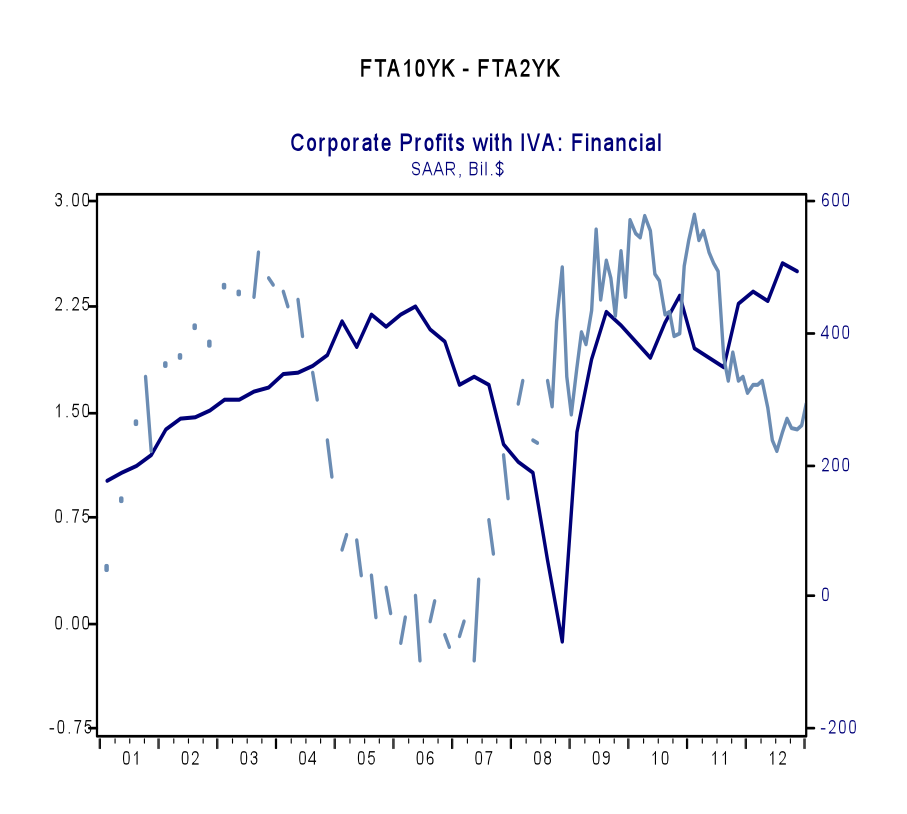
\includegraphics[scale=.70]{figure/InvertedTbill2.png}\\[-0.7cm]
\caption{Profits Falling Before the Recession\label{fig:profFall}}
\end{figure}

Figure \ref{fig:profFall} shows the inverted yield curve, and lagging financial corporate profits.  It is important that the financial corporate profits lag the inverted yield, and interestingly the financial corporate profits peak at the deepest inversion treasury curve.  In the years leading up to the current financial crisis, banks around the world expanded their balance sheets to increase profitability in an environment of cheap funding.\cite{Kunt}  The financial firms did not pull back on investing, even in the face of an inverted yield curve which had prefaced every recession since 1964.  


%%%%%%%%%%%%%%%%%%%%%%%%%%%%%%%%%%%%%%%%%%%%
\pagebreak
\subsubsection{Response of Firms}

\begin{figure}[H]
\centering
\begin{subfigure}{.5\textwidth}
  \centering
  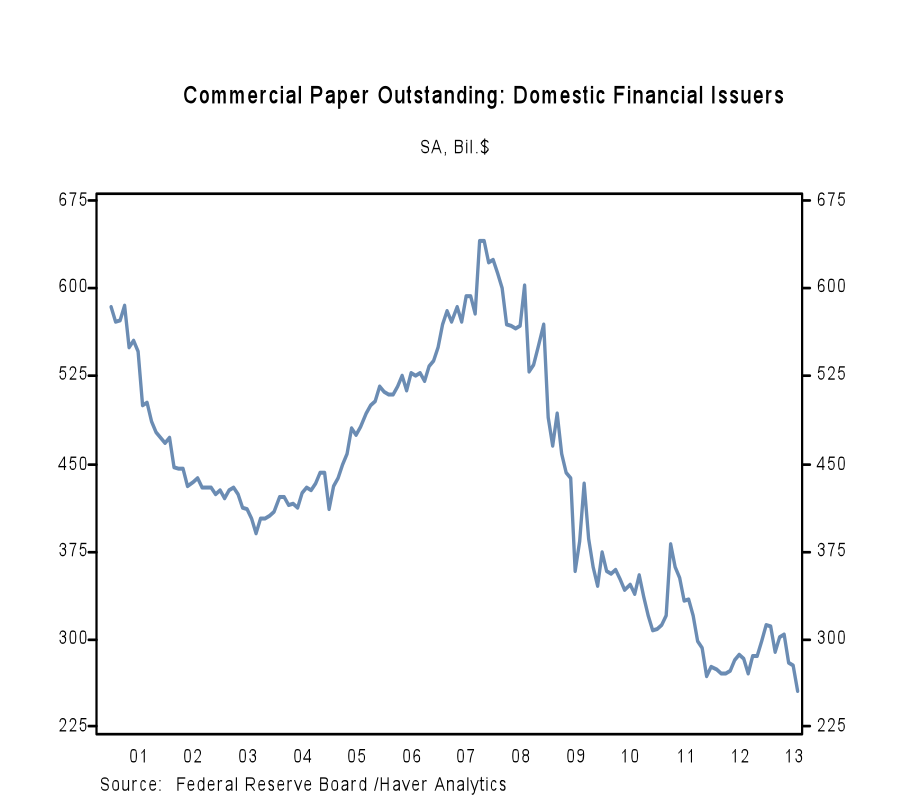
\includegraphics[width=1.0\linewidth]{figure/DomesticFinancial_CommPaper.png}
  \caption{Commercial Paper in Short-Term}
   \label{fig:FinComm}
\end{subfigure}%
\begin{subfigure}{.5\textwidth}
  \centering
  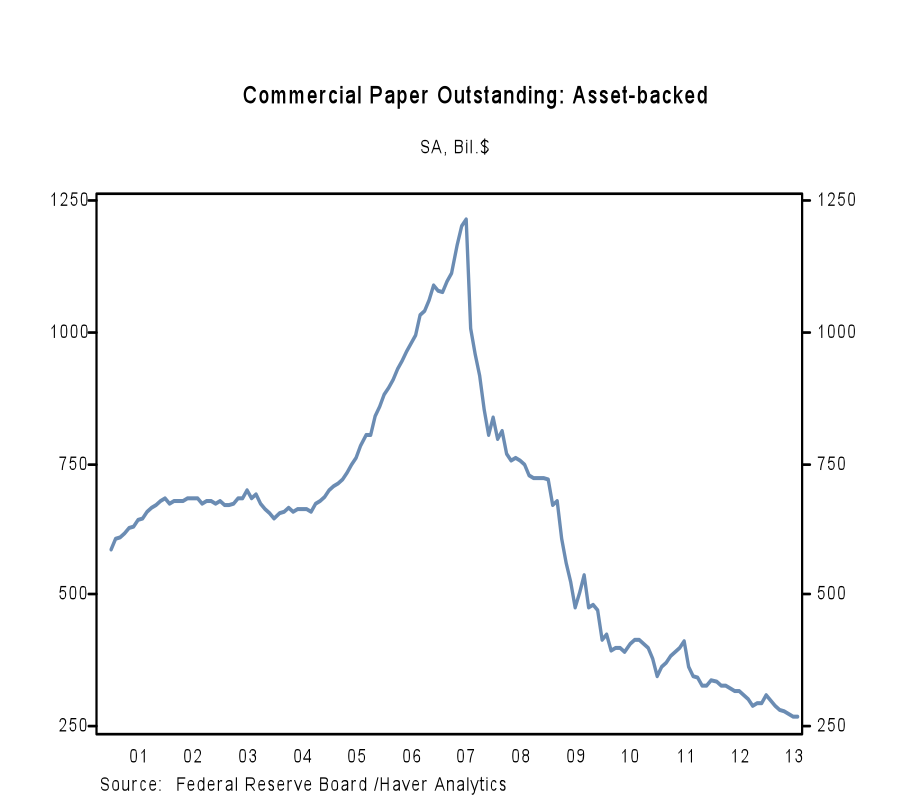
\includegraphics[width=1.0\linewidth]{figure/CommPaperOut_AssetBacked.png}
  \caption{New Short-Term Funding Pool }
  \label{fig:FinABS}
\end{subfigure}
\caption{Leverage Funding Before Financial Crisis}
\label{fig:LeverageFinance}
\end{figure}

These short-term funding markets exist so that private firms can make some interest on excess reserve cash.  The private firm holding excess reserve cash, that may want to remain liquid for a period of time, can find other financial firms that need short-term cash to meet overnight requirements.  Typically commercial paper, seen in subfigure \ref{fig:FinComm} and subfigure \ref{fig:FinABS}, is lent out with a duration of no more than 270 days.  In leveraged investing, short-term funding may be required to meet federal reserve requirements.  

Commercial paper that is exchanged without collateral has existed and been used in many tumultuous economic periods.  Asset-backed commercial paper was introduced to protect lenders of excess reserves from having a short-term financial firm loan default.  The likelihood of this type of financial firm failure, in less than 270 days, has increased with the prevalence of leveraged and hedging investment.  Long Term Capital Management was a particularly famous hedge fund that collapsed in a commercial paper maturity period.  The build up of outstanding typical commercial paper prior to the 2008 financial crisis (subfigure \ref{fig:FinComm}) was not unlike the build up of outstanding commercial paper before the dot com bubble.  Interestingly the quantity of outstanding asset-backed commercial paper (subfigure \ref{fig:FinABS}) exploded prior to the financial crisis of 2008.  The correlating peaks of these two short-term lending metrics are indicative of the massive leverage and push for profitability entering the financial crisis. 



\subsection{Short-Term Funding: Greater Leverage in Crisis}

Within a margin account the credit balance of the account includes not only the cash remaining in the account, but also proceeds from short sales along with money used to meet margin requirements.  The investment manager must hold additional funds in a margin account if the account is being leveraged.

\begin{figure}[H]
\centering
\begin{subfigure}{.5\textwidth}
  \centering
  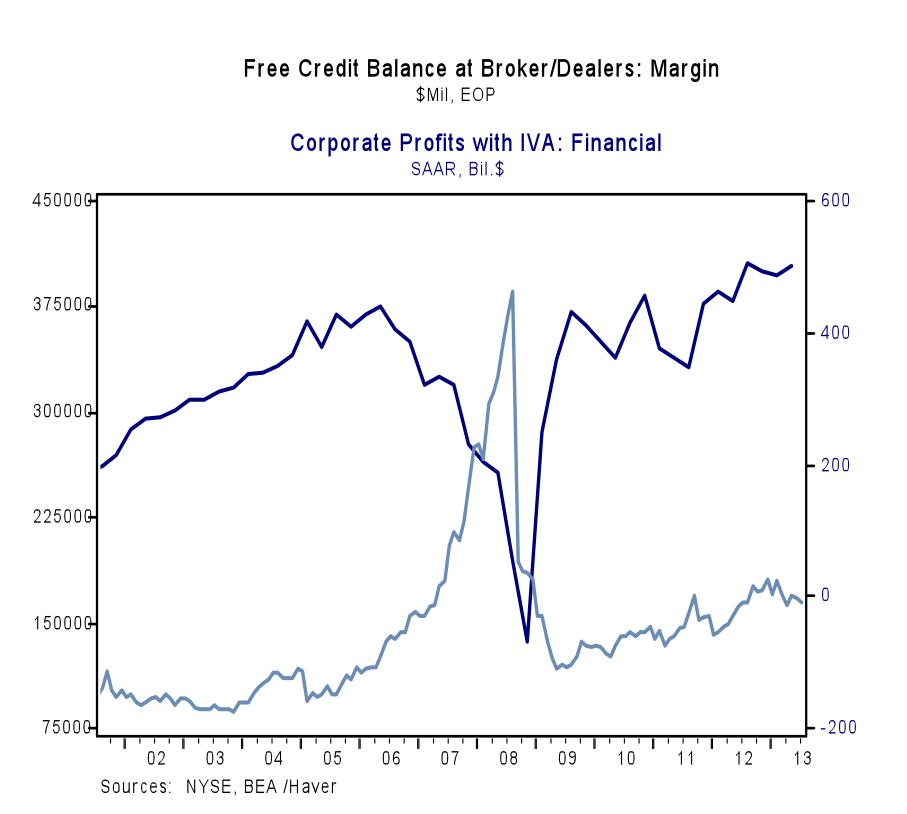
\includegraphics[width=1.0\linewidth]{figure/Profits_and_FreeCredit.png}
  \caption{Leveraging in Profit Squeeze }
  \label{fig:leveraging}
\end{subfigure}%
\begin{subfigure}{.5\textwidth}
  \centering
  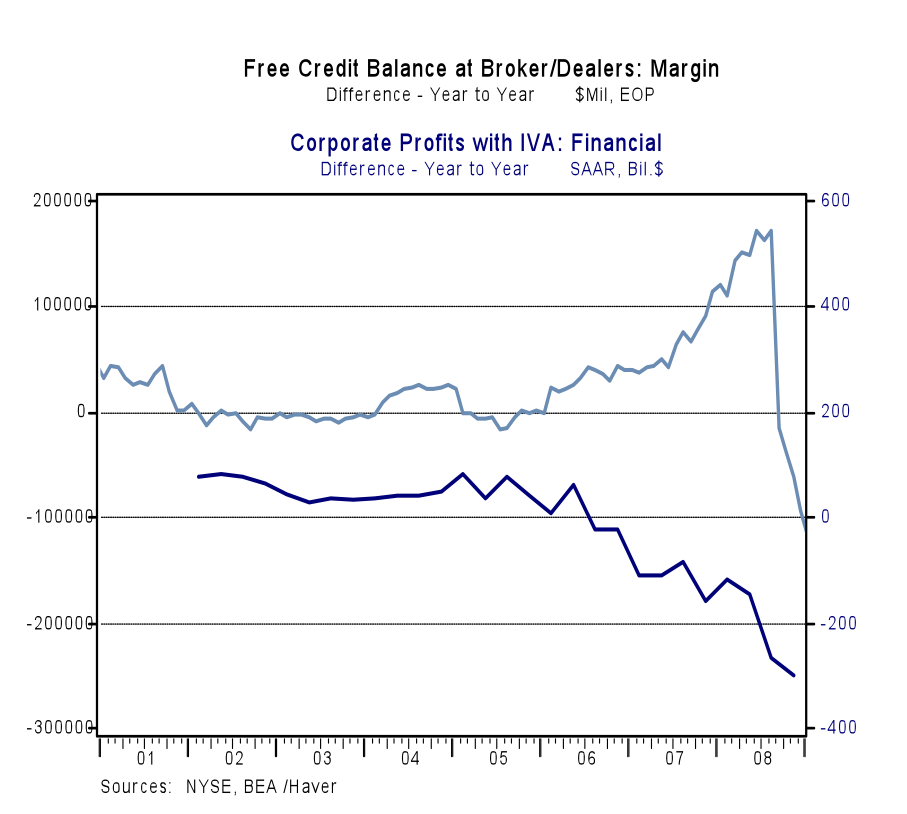
\includegraphics[width=1.0\linewidth]{figure/DiffYearProfits_and_FreeCredit2.png}
  \caption{Attempts to Offset Losses}
  \label{fig:protectLosses}
\end{subfigure}
\caption{Larger Margin Required in Leveraged Client Accounts}
\label{fig:marginGrowth}
\end{figure}

Figure \ref{fig:marginGrowth} shows the rise of margin accounts within the free credit balance.  The growth of margin accounts correlates strongly with the fall of financial corporate profits.  Margin accounts support leveraged transactions and if they are growing, so to is the amount of leverage and speculation.  Financial firms make their profits from speculation, and their portfolios are often highly risky ... Leverage increases the potential profits of shareholders and fee commissioning financial corporates ... it also increases shareholder's risks: the greater the leverage, the bigger the profit to shareholders and fee commissioning financial corporates if investments are successful, but the bigger the loss to \textit{only} shareholders if investments are not successful.\cite{Dowd}  

 
\begin{figure}[H]
\centering
\begin{subfigure}{.5\textwidth}
  \centering
  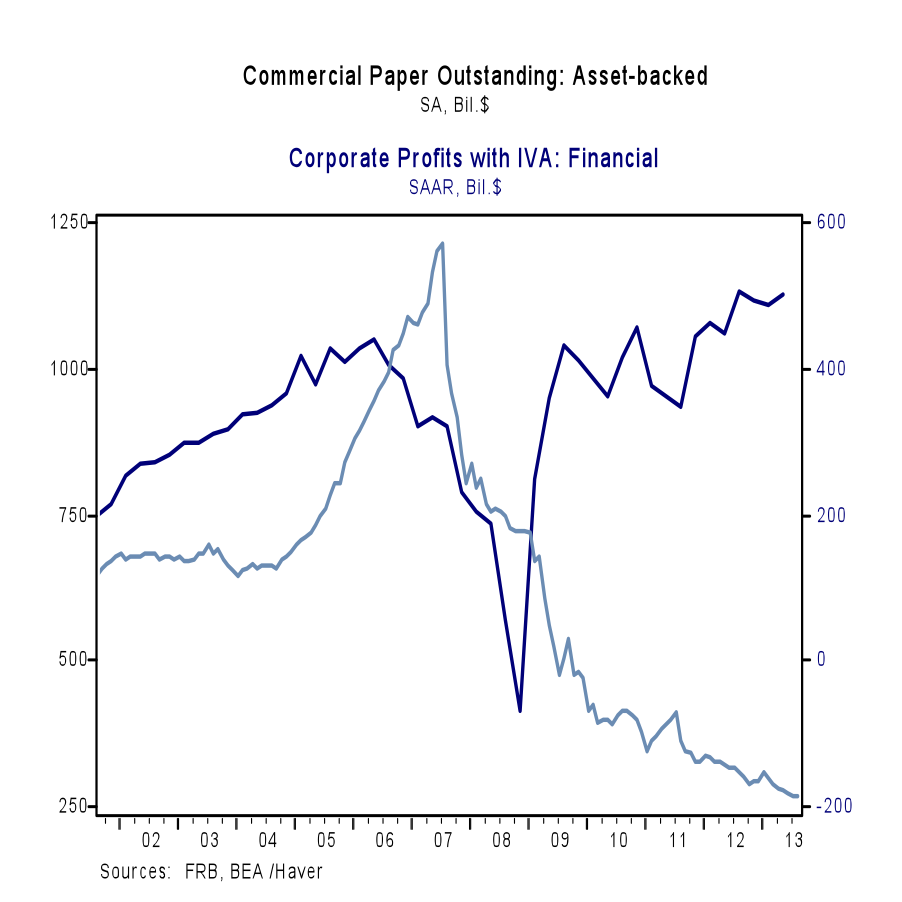
\includegraphics[width=1.0\linewidth]{figure/CommPaper_FinProfits.png}
  \caption{Increased Volume of Short-Term Lending}
  \label{fig:shortTermLend}
\end{subfigure}%
\begin{subfigure}{.5\textwidth}
  \centering
  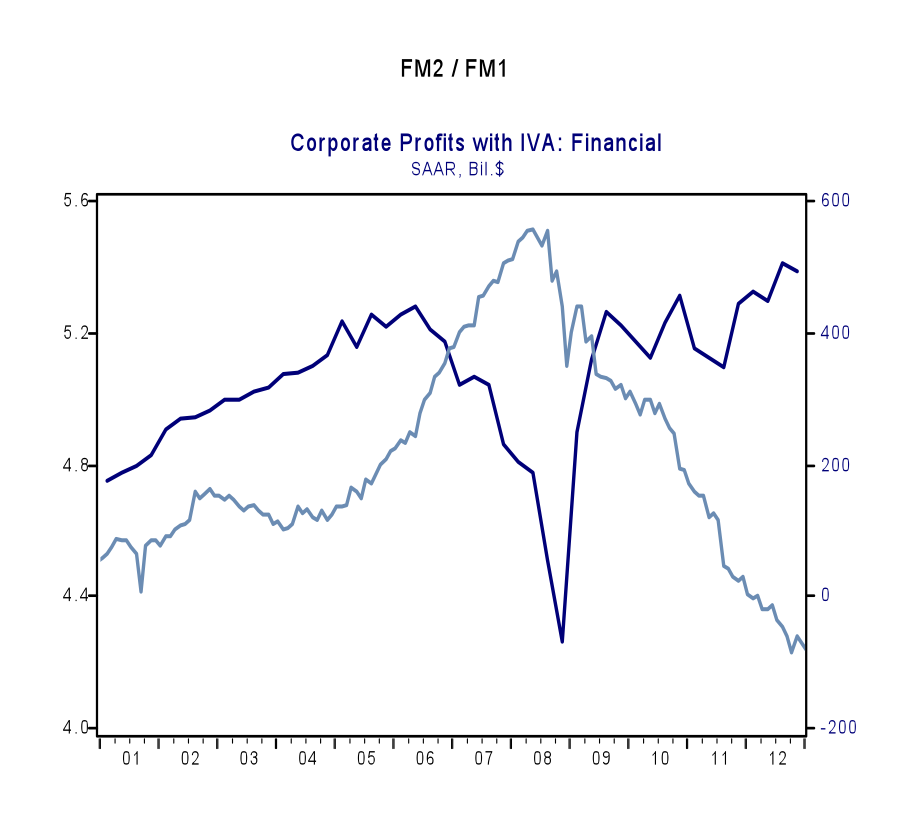
\includegraphics[width=1.1\linewidth]{figure/M2Peak2.png}
  \caption{Investment Peak: Market Wide }
  \label{fig:M2Peak}
\end{subfigure}
\caption{Striving for Profitability}
\label{fig:NEW2}
\end{figure}

As corporate profits started to reverse their course in 2006, the banks pushed ever harder to maintain an artificially high rate of profit.  All the extra leverage helped spike the use of asset-backed commercial paper, and accelerate the growth of M2 with respect to M1 money supply.

Corporate profits are a better illustration of broad investment choices after the repeal of Glass-Steagall.  In this financial crisis, leverage was applied to maintain not only client wealth, but to protect and gain for the corporation and its employees.  It is not clear whether the treasury curve inversion exacerbated the decline in financial profitability, but the financial market response to push leveraging strategies even harder clearly shook the stability of market assets.

%%That EXTRA short-term funding that is not coming from the FED is going into time sensitive debt instruments, and boosting M2 in the face of a recession....very BAD

%Inversion as Catalyst for Leverage in Profit Squeeze
 % The Broker is leveraging more and needs to meet minimum requirements%
%Larger Margin Required in Client Accounts


%%
%%
%%%%%%%%%\pagebreak
%%%%%%%%%\subsubsection{Intended Purpose of Short-Term Debt}
%%%%%%%%%What SHORT TERM FINANCING IS SUPPOSED TO BE USED FOR!!!! in crisis borrowing, but they try to obscure it in the private markets, so that the fed doesn't see.  
%%%%%%%%%%%They are supposed to borrow when things go bad, but they do so in the Fed Funds market.....when they try to obscure, we get the inflated borrowing in the two other graphs.
%%%%%%%%%
%%%%%%%%%\begin{figure}[H]
%%%%%%%%%\centering
%%%%%%%%%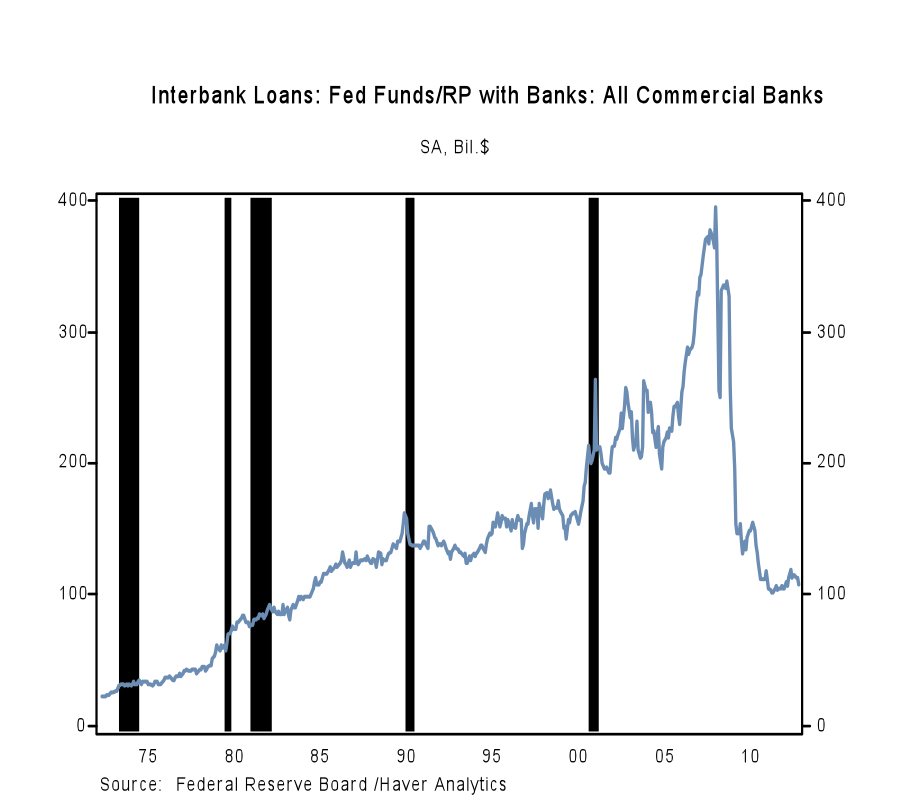
\includegraphics[scale=.70]{figure/interbankFedAllComm.png}\\[-0.7cm]
%%%%%%%%%\caption{Borrowing to Meet Requirements \& Crisis Borrowing\label{fig:FedOut}}
%%%%%%%%%\end{figure}
%%%%%%%%%
%%%%%%%%%

